\documentclass[12pt,a4paper]{article}
\usepackage[top=1.5cm, bottom=1.5cm, left=2.0cm, right=1.5cm] {geometry}
\usepackage{amsmath,amssymb,txfonts}
\usepackage{tkz-euclide}
\usepackage{setspace}
\usepackage{lastpage}

\usepackage{tikz,tkz-tab}
%\usepackage[solcolor]{ex_test}
%\usepackage[dethi]{ex_test} % Chỉ hiển thị đề thi
\usepackage[loigiai]{ex_test} % Hiển thị lời giải
%\usepackage[color]{ex_test} % Khoanh các đáp án
\everymath{\displaystyle}

\def\colorEX{\color{purple}}
%\def\colorEX{}%Không tô màu đáp án đúng trong tùy chọn loigiai
\renewtheorem{ex}{\color{violet}Câu}
\renewcommand{\FalseEX}{\stepcounter{dapan}{{\bf \textcolor{blue}{\Alph{dapan}.}}}}
\renewcommand{\TrueEX}{\stepcounter{dapan}{{\bf \textcolor{blue}{\Alph{dapan}.}}}}

%---------- Khai báo viết tắt, in đáp án
\newcommand{\hoac}[1]{ %hệ hoặc
    \left[\begin{aligned}#1\end{aligned}\right.}
\newcommand{\heva}[1]{ %hệ và
    \left\{\begin{aligned}#1\end{aligned}\right.}

%Tiêu đề
\newcommand{\tenso}{iMath}
\newcommand{\tentruong}{Phần mềm tạo đề tự động}
\newcommand{\tenkythi}{ĐỀ ÔN TẬP TOÁN 12}
\newcommand{\tenmonthi}{Môn thi: Toán}
\newcommand{\thoigian}{}
\newcommand{\tieude}[2]{
    \noindent
    %Trái
    \begin{minipage}[b]{7cm}
        \centerline{\textbf{\fontsize{13}{0}\selectfont \tenso}}
        \centerline{\textbf{\fontsize{13}{0}\selectfont \tentruong}}
        \centerline{(\textit{Đề thi có #1\ trang})}
    \end{minipage}\hspace{1.5cm}
    %Phải
    \begin{minipage}[b]{9cm}
        \centerline{\textbf{\fontsize{13}{0}\selectfont \tenkythi}}
        \centerline{\textbf{\fontsize{13}{0}\selectfont \tenmonthi}}
        \centerline{\textit{\fontsize{12}{0}\selectfont Thời gian làm bài: \thoigian\ phút}}
    \end{minipage}
    \begin{minipage}[b]{10cm}
        \textbf{Họ và tên HS: }{\tiny\dotfill}
    \end{minipage}
    \begin{minipage}[b]{8cm}
        \hspace*{4cm}\fbox{\bf Mã đề: #2}
    \end{minipage}\vspace{3pt}
}
\newcommand{\chantrang}[2]{\rfoot{Trang \thepage $-$ Mã đề #2}}
\pagestyle{fancy}
\fancyhf{}
\begin{document}
%Thiết lập giãn dọng 1.5cm 
%\setlength{\lineskip}{1.5em}
%Nội dung trắc nghiệm bắt đầu ở đây


\tieude{\pageref{LastPage}}{001}

\chantrang{\pageref{LastPage}}{001}

\setcounter{page}{1}

\setcounter{ex}{0}
\Opensolutionfile{ans}[ans/ans001]
\begin{ex}
 Cho hàm số $y=f(x)$ xác định trên $\mathbb{R}$ và có bảng biến thiên như hình vẽ sau:


 
\begin{center}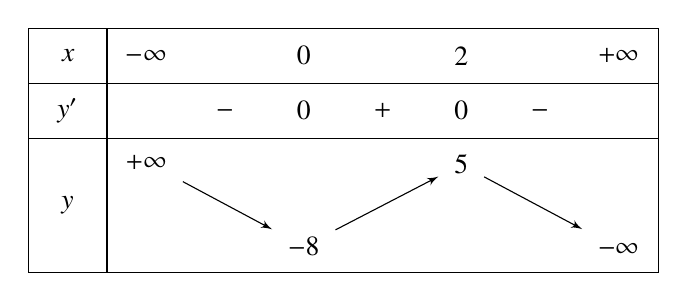
\begin{tikzpicture}
             \tkzTabInit[nocadre=false, lgt=1, espcl=2] 
             {$x$ /0.7,$y'$ /0.7,$y$ /1.7}
             {$-\infty$,$0$,$2$,$+\infty$}
             \tkzTabLine{,-,0,+,0,-,} 
             \tkzTabVar{+/$+\infty$ ,-/ $-8$, +/ $5$ /, -/$-\infty$ /} 
            \end{tikzpicture}
\end{center}
Điểm cực đại của hàm số $y=f(x)$ bằng
\choice
{ ${5}$ }
   { \True ${2}$ }
     { ${0}$ }
    { ${-8}$ }
\loigiai{ 

 Điểm cực đại của hàm số $y=f(x)$ bằng ${2}$. 
 }\end{ex}


 \begin{center}
-----HẾT-----
\end{center}

 \Closesolutionfile{ans}
% \newpage
% BẢNG ĐÁP ÁN MÃ ĐỀ 001
% \inputansbox{2}{ans/ans001}


\end{document}